\clearpage
\subsection{Direct shear with prescribed velocity}
\label{sec:direct-shear-verification}

\subsubsection*{Problem and verification objective}

This example checks the constant prescribed-velocity condition in a direct shear test with a flat frictional interface. Both the normal-loading and shearing stages use a 5 mm grid. The velocity condition is applied to a strip of material points near the top of the upper block. The verification compares their saved velocities and displacements with the imposed motion.

The specimen consists of two elastic blocks, each 100 mm long in X and 10 mm thick in Y. The lower block occupies $0\leq z\leq25$ mm and the upper block $25\leq z\leq55$ mm. Both extend from $x=10$ to $110$ mm. The mesh contains $24\times2\times12$ cubic cells of side 5 mm. The two blocks contain 3,520 material points in total.

The material has Young's modulus $E=5$ GPa, Poisson's ratio $\nu=0.25$, and density $\rho=2600$ kg/m$^3$. Gravity is zero. The Y boundary planes prevent normal motion and allow tangential motion. The X boundary planes and the upper Z plane are free.

A downward load of 1,000 N is distributed over the upper 5 mm of the specimen. The initial interface area is $A_0=0.100\times0.010=0.001$ m$^2$, giving a nominal normal stress of 1 MPa. During shearing, material contact is active with friction coefficient $\mu=0.6$ and collinear contact normals.

\subsubsection*{Normal loading and transfer of stresses}

The first stage runs for 0.005 s with kinetic damping, material contact disabled, and a sliding boundary at the bottom Z plane. It prepares the initial stresses under the normal load. This is a single-phase mechanical equilibration stage.

Figure~\ref{fig:direct-shear-consolidation} shows the mean compressive vertical stress and the kinetic energy during this stage. The mass-weighted stress average excludes the 320 particles in the loaded layer, selected in the reference configuration by the load box ($50\leq z\leq55$ mm). The remaining 3,200 particles give a mean compression of 1.00004 MPa in the last particle output, differing from the nominal applied stress of 1 MPa by approximately 0.0037\%. The same particle selection is used throughout both stages.

The kinetic energy decreases from a recorded maximum of $9.07\times10^{-5}$ J to $1.57\times10^{-30}$ J in the last energy record. This decrease supports using the resulting stress field as the initial state for shearing. The shearing input recreates the same particle geometry and imports the stress tensors of all 3,520 particles.

\begin{figure}[H]
    \centering
    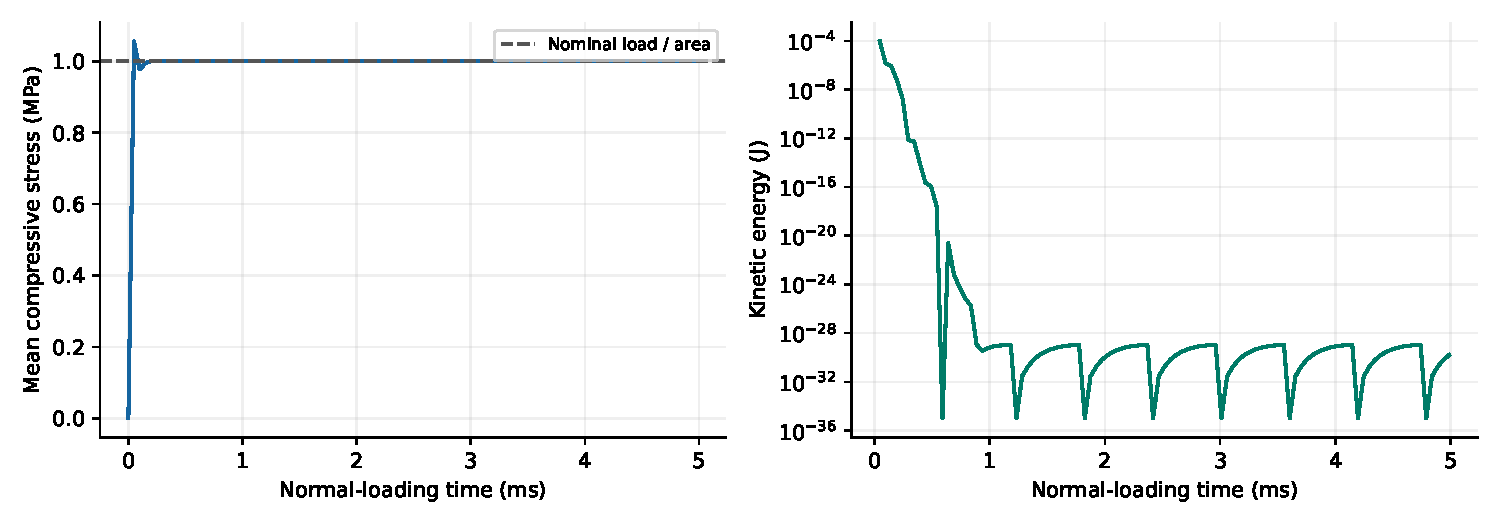
\includegraphics[width=\textwidth]{figures/direct-shear-consolidation.pdf}
    \caption{Normal-loading stage: mean compressive vertical stress excluding the loaded layer, and total kinetic energy from the saved results.}
    \label{fig:direct-shear-consolidation}
\end{figure}

\subsubsection*{Input file}

The complete shearing input is listed below. The changes needed for normal loading are described after the listing. The normal stress file must first be generated by the normal-loading stage.

The shearing stage uses USL integration, no damping, and a duration of 0.05 s. Its bottom Z boundary is fixed. The selected strip belongs to body 2 and lies within $20\leq x\leq100$ mm, $0\leq y\leq10$ mm, and $52.5\leq z\leq55$ mm in the reference configuration. This selects 128 particles. Only their X velocity is prescribed; \texttt{null} leaves the other components unconstrained by this condition.

\begin{lstlisting}[basicstyle=\ttfamily\footnotesize,caption={Complete input for the shearing stage.},label={lst:direct-shear-input}]
{
  "time": 0.05,
  "critical_time_step_multiplier": 0.3,
  "stress_scheme_update": "USL",
  "n_threads": 4,
  "n_phases": 1,
  "gravity": [0, 0, 0],
  "results": {
    "print": 100,
    "material_point_results": ["id", "body", "mass", "active", "displacement", "velocity", "stress"],
    "grid_nodal_results": ["id", "contact_force", "mass_gradient_vector", "prescribed_velocity_reaction"]
  },
  "mesh": {
    "cells_dimension": [0.005, 0.005, 0.005],
    "cells_number": [24, 2, 12],
    "origin": [0, 0, 0],
    "boundary_conditions": {
      "plane_X0": "free",
      "plane_Xn": "free",
      "plane_Y0": "sliding",
      "plane_Yn": "sliding",
      "plane_Z0": "fixed",
      "plane_Zn": "free"
    }
  },
  "material": [
    {
      "type": "elastic",
      "id": 1,
      "young": 5000000000.0,
      "density": 2600,
      "poisson": 0.25
    }
  ],
  "body": [
    {
      "type": "polygon_2d",
      "id": 1,
      "material_id": 1,
      "extrude_direction": "y",
      "extrude_displacement": 0.01,
      "discretization_length": 0.005,
      "points": [
        [0.01, 0, 0],
        [0.11, 0, 0],
        [0.11, 0, 0.025],
        [0.01, 0, 0.025]
      ]
    },
    {
      "type": "polygon_2d",
      "id": 2,
      "material_id": 1,
      "extrude_direction": "y",
      "extrude_displacement": 0.01,
      "discretization_length": 0.005,
      "points": [
        [0.01, 0, 0.025],
        [0.11, 0, 0.025],
        [0.11, 0, 0.055],
        [0.01, 0, 0.055]
      ]
    }
  ],
  "load_distributed_box": [
    {
      "point_p1": [0.01, 0, 0.05],
      "point_p2": [0.11, 0.01, 0.055],
      "load": [0, 0, -1000]
    }
  ],
  "damping": {
    "type": "none"
  },
  "save_state": true,
  "save_state_file": "final-stress.json",
  "load_state": true,
  "load_state_file": "../01-normal-loading/normal-stress.json",
  "prescribed_velocity": [
    {
      "body_id": 2,
      "point_p1": [0.02, 0, 0.0525],
      "point_p2": [0.1, 0.01, 0.055],
      "velocity": [0.01, null, null]
    }
  ],
  "material_contact": {
    "active": true,
    "pairs": [
      {
        "id": 1,
        "friction": 0.6,
        "normal_type": "collinear",
        "master_body_id": 1,
        "slave_body_id": 2
      }
    ]
  }
}
\end{lstlisting}

For normal loading, use the same geometry, material, normal load, and output interval, with the following changes to the shearing input. Remove \texttt{prescribed\_velocity}, \texttt{load\_state}, and \texttt{load\_state\_file}. The nodal output \texttt{prescribed\_velocity\_reaction} is also omitted. Set the remaining stage-specific entries as follows:

\begin{lstlisting}[basicstyle=\ttfamily\footnotesize]
"time": 0.005,
"damping": {"type": "kinetic"},
"save_state": true,
"save_state_file": "normal-stress.json"
// Inside mesh.boundary_conditions:
"plane_Z0": "sliding"
// Inside material_contact:
"active": false
// Inside material_contact.pairs[0]:
"normal_type": "master"
\end{lstlisting}

\subsubsection*{Verification of the imposed motion}

For every selected particle, the expected motion during shearing is
\begin{equation}
    v_{xp}^{k+1/2}=\bar v_x=0.01\ \mathrm{m/s},\qquad
    x_{xp}^{k+1}-x_{xp}^{0}=\bar v_x(t^k+\Delta t).
    \label{eq:direct-shear-expected-motion}
\end{equation}
The nominal displacement after 0.05 s is therefore 0.5 mm. The comparison uses the particle selection in the input.

The saved series contains an initial state and 100 subsequent particle outputs. In every subsequent output, the minimum and maximum X velocities over the 128 selected particles are both 0.01 m/s. The maximum absolute velocity error is zero at the precision of the exported files. The initial output precedes enforcement of the velocity condition and is excluded from this velocity-error check. The displacement follows the same imposed motion, as shown in Figure~\ref{fig:direct-shear-velocity-check}. 
\begin{figure}[H]
    \centering
    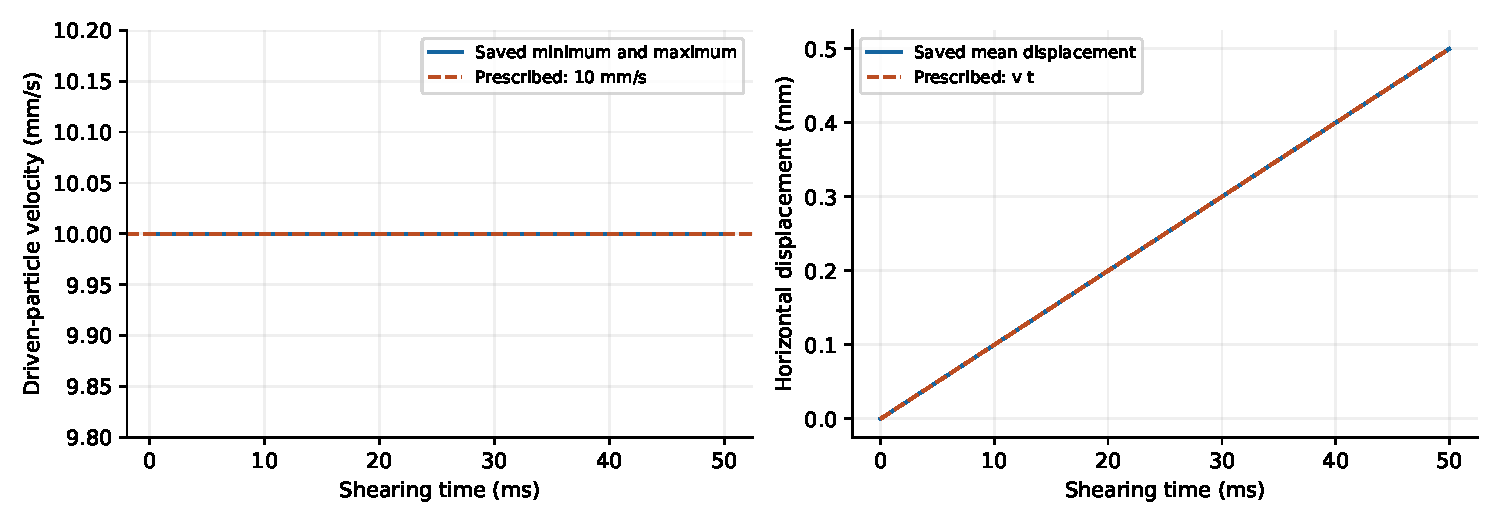
\includegraphics[width=\textwidth]{figures/direct-shear-velocity-check.pdf}
    \caption{Imposed-motion check on the 128 selected particles: saved velocity bounds and mean displacement compared with the prescribed values. The velocity bounds coincide.}
    \label{fig:direct-shear-velocity-check}
\end{figure}

\subsubsection*{Shear stress and vertical displacement}

Figure~\ref{fig:direct-shear-response} presents the response for $h=5$ mm and $v=0.01$ m/s. The shear stress is calculated from the summed horizontal prescribed-velocity reaction divided by the initial interface area.

\begin{figure}[H]
    \centering
    \includegraphics[width=\textwidth]{figures/direct-shear-response.pdf}
    \caption{Shear stress and relative vertical displacement during shearing.}
    \label{fig:direct-shear-response}
\end{figure}
